\section{Experimental Analysis of \sahad{}, \ensahad{} \& \harpsahad{}}
\label{sec:experiment}

We carry out a detailed experimental analysis of  \sahad{}, \ensahad{} and
\harpsahad{}. We focus on three aspects:

({\it i}) \emph{Quality of the solution}:
We compare the color coding results with exact count on small graphs in order to
measure the empirical approximation error of our algorithms and show that the
error is very small (less than 0.5\% with one iteration as shown in
Figure~\ref{fig::error}) so in the following experiments we run the program for
a single iteration;

({\it ii}) \emph{Scalability of the algorithms as a function of
template size, graph size and computing resources:}
We carried out experiments using templates with size ranging from 3 nodes to 12
nodes, including both labeled and unlabeled templates. The graphs we use go from
several hundreds of thousands of nodes to tens of millions. We also study how
our algorithm scales in terms of computing resources including number of threads
per node, number of computing nodes, different settings of mappers and reducers,
etc.

({\it iii}) \emph{Variations of the problem:}
Our framework has the ability to extend to a variety of measurements related
with the subgraph counting problem. In the experiments, we show the
unlabled/labeled subgraph counting and graphlet distribution results.

({\it iv}) \emph{Enhancing overall performance by system tuning:}
We also investigate different components of the system and their impact to the
overall performance. For example, \ensahad{} studies the communication and
sorting cost in the intermediate stage of the system and gives approaches for
improvement. We also propose a degree based graph partitioning scheme that can
improve the performance of Harp by imposing better load balancing in terms of
computations within each partition.  Table~\ref{tab:exp-summary} listed main
results we obtained with various methods.

\begin{table}[hptb]
	\caption{Comparison on \sahad{}, \ensahad{} and \harpsahad{}}
\label{tab:exp-summary}
\centering{
\begin{tabular}{c|c|c|c}
\hline
Method & Networks & Templates & Performance \\
\hline
\sahad{} & 268M edges & $\leq$ 12 nodes & \vtop{\hbox{\strut 10s of min for 7 node}\hbox{\strut template on Chicago}}   \\
\hline
\ensahad{} & 12M edges & 5 nodes & \vtop{\hbox{\strut 20\% improvement}\hbox{\strut over \sahad{}}} \\
\hline
\harpsahad{} & 1.2B edges & upto 7 nodes & \vtop{\hbox{\strut 7 - 8 times faster}\hbox{\strut than \sahad{}}} \\
\hline
\end{tabular}
}
\end{table}


\subsection{Experimental Design}
\label{sec:datasets-comp}

\subsubsection{Datasets}

For our experiments, we use synthetic social contact networks of the following
cities and regions: Miami, Chicago, New River Valley (NRV), and New York City
(NYC) (see~\cite{barrett2009generation} for detains). We consider demographic
labels -- \{kid, youth, adult, senior\} (based on the age) and gender for
individuals.  We also run experiments on a $G(n,p)$ graph (denoted GNP100) with
$n$ nodes, each pair of nodes connected with probability $p$, and randomly
assigned node labels. We also experiment on few other networks:
Web-Google~\cite{snap}, RoadNet (rNet)~\cite{snap}, Twitter~\cite{Kwak10www} and Chung-Lu random
graphs~\cite{chung2002connected}.  Table~\ref{tab:dataset} summarizes the
characteristics of the networks.

\begin{table}[hptb]
\caption{Networks used in the experiments}
\label{tab:dataset}
\centering{
\begin{tabular}{c|c|c}
\hline
Network & No. of Nodes(in million) & No. of Edges(in million) \\
\hline
Twitter & $41.7$ & $1202.5$ \\
Miami & $2.1$ & $52.7$ \\
Chicago & $9.0$ & $268.9$ \\
NYC & $18.0$ & $480.0$ \\
NRV & $0.2$ & $12.4$ \\
rNet & $2.0$ & $2.8$ \\
GNP100 & $0.1$ & $1.0$ \\
Web-Google & $0.9$ & $4.3$ \\
\hline
\end{tabular}
}
\end{table}

\subsubsection{Templates}
The templates we use in the experiments are shown in Figure
~\ref{fig:templates}. The templates vary in size from $5$ to $12$
nodes, in which \emph{U5-1,}$\ldots$\emph{U10-1} are the unlabeled templates
and \emph{L7-1} ,\emph{L10-1} and \emph{L12-1} are the labeled templates. In
the labels, \emph{m}, \emph{f}, \emph{k}, \emph{y}, \emph{a} and \emph{s} stand
for \emph{male}, \emph{female}, \emph{kid}, \emph{youth}, \emph{adult} and
\emph{senior}, respectively.

\begin{figure}[htbp]
\centerline{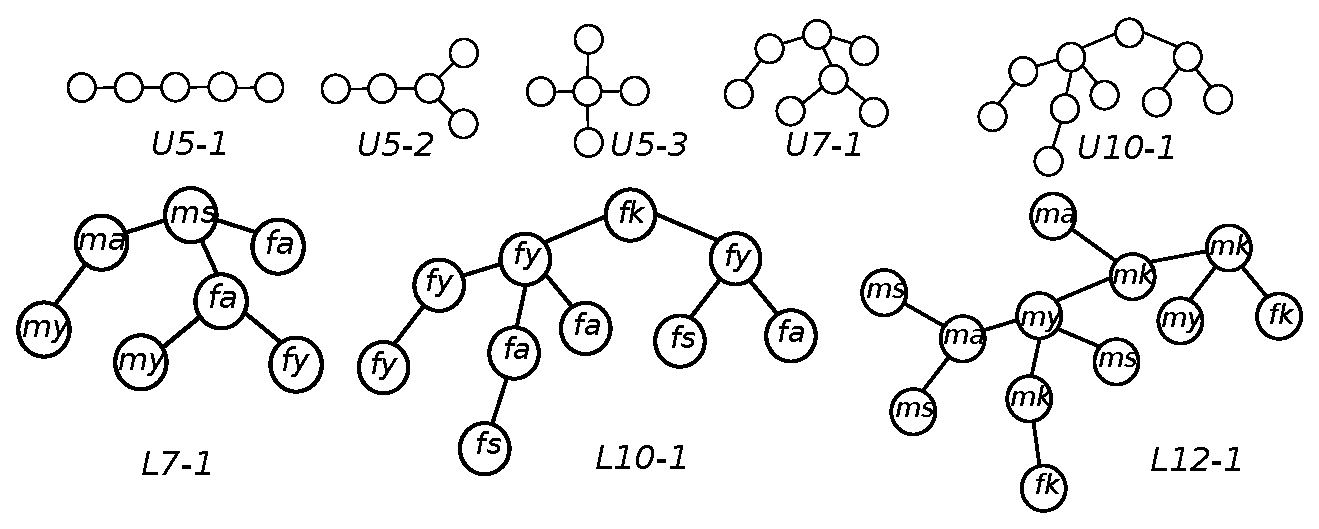
\includegraphics[width=0.45\textwidth]{plots/templates.eps}}
\caption{Templates used in the experiments.}
\label{fig:templates}
\end{figure}

\subsubsection{Computing Environment}
For experiments with \sahad{}, we use a computing cluster \textbf{Athena},
with $42$ computing nodes and a large RAM memory footprint.  Each node has a
quad-socket AMD 2.3GHz Magny Cour 8 Core Processor, i.e., $32$ cores per node or
$1344$ cores in total, and $64$ GB RAM(12.4 TFLOP peak). The local disk
available on each node is $750GB$.  Therefore, we can have maximum $31.5TB$
storage for the HDFS. In most of our experiments, we use up to $16$ nodes, which
give up to $12TB$ capacity for the computation. Although the number of cores and
RAM capacity on each node can support a large number of mappers/reducers, the
availability of a single disk on each node limits aggregate I/O bandwidth of all
parallel processes on each node. To make it worse, aggregate I/O bandwidth of
parallel processes doing sequential I/O could result in many extra disk seeks
and hurt overall performance. Therefore, disk bandwidth is the bottleneck for
more parallelism in each node. This limitation is further discussed in
section~\ref{sec:perf}. We also use the public Amazon Elastic Computing Cloud
(\textbf{EC2}) for some of our experiments. EC2 enables customers to instantly
get cheap yet powerful computing resources, and start computing business with no
upfront cost for hardware. We allocated 4 \emph{High-CPU Extra-Large} instances
from EC2. Each instance has $8$ cores, $7~GB$ RAM, and two $250~GB$ virtual
disks (Elastic Block Store Volume).

For experiments with \harpsahad{}, we use Juliet cluster (Intel Haswell architectures)
with 1,2,4,8 and 16 nodes.  Juliet cluster contains 32 nodes each with two
18-core 36-thread Intel Xeon E5-2699 processors and 96 nodes each with two
12-core 24-thread Intel Xeon E5-2670 processors. All the nodes used in the
experiments are with Intel Xeon E5-2670 processors and $128~GB$ memory. All the
experiments are performed on standard cooper $1~Gbps$ Ethernet. 

\subsubsection{Performance metrics}
We carry out experiments on \sahad{}, \ensahad{} and
\harpsahad{}. For \sahad{}, we measure the approximation bounds, the impact of
Hadoop configuration including number of Mapper/Reducers and performance on
queries related with various templates and graphs. For enhanced \sahad{},
we measure the performance improvement gained by eliminating the sorting in the
intermediate stage. We also measures the impact with difference partitioning
schemes. Then with Harp, similar to \sahad{}, we measure the performance
impact with various templates and graphs, as well as the system performance
regarding number of computing nodes. We also compare \harpsahad{} and \sahad{} to
study the improvement Harp brings. 

\subsection{Performance of \sahad{}}
In this section, we evaluate various aspects of the performance.  Our main
conclusions are summarized below. Table~\ref{tab:results} summarizes the
different experiments we perform, which are discussed in greater details later.

\smallskip
\textbf{1. Approximation bounds}: While the worst case bounds on the algorithm
imply $O(e^k\log{(1/\delta)}\frac{1}{\varepsilon^2})$ rounds to get an
$(\varepsilon,\delta)$-approximation (see Lemma~\ref{lemma:workcomp}), in
practice, we find that far fewer iterations are needed.

\smallskip
\textbf{2. System performance}: We run our algorithm on a diverse set of
computing resources, including the publicly available Amazon EC2 cloud. We find
our algorithm scales well with the number of nodes, and disk I/O is one of the
main bottlenecks.  \emph{We posit that employing multiple disks per node (a
rising trend in Hadoop) or using I/O caching will help mitigate this bottleneck
and boost performance even further.}

\smallskip
\textbf{3. Performance on various queries}: We evaluate the performance on
templates with sizes ranging from 5 to 12. We find labeled queries are
significantly faster than unlabeled ones, and the overall running time is under
35 minutes for these queries on our computing cluster (described below). We also
get comparable performance on EC2.

\begin{table*}[hptb]
  \caption{Summary of the experiment results (refer to Section~\ref{sec:datasets-comp} for the terminology used
in the table)}

\label{tab:results}
\centering{
\begin{tabular}{l|l|p{8pc}|p{12pc}}
\hline
\textbf{Experiment} & \textbf{Computing resource} & \textbf{Template \& Network} &
\textbf{Key Observations} \\

\hline
Approximation bounds & Athena & U7-1 \& GNP100 & error well below 0.5\% \\

\hline
Impact of the number of data nodes & Athena & U10-1 \& Miami, GNP100 & scale from 4
hours to 30 minutes with data nodes from 3 to 13\\

\hline
Impact of the number of concurrent reducers & Athena \& EC2 & U10-1 \& Miami &
performance worsen on Athena \\

\hline
Impact of the number of concurrent mappers & Athena \& EC2 & U10-1 \& Miami & no
apparent performance change \\

\hline
Unlabeled/labeled templates counting & Athena \& EC2 & templates from
Figure~\ref{fig:templates} and networks from Table \ref{tab:dataset} & all tasks
complete in less than 35 minutes \\

\hline
Graphlet frequency distribution & Athena & U5-1 \& Miami,Chicago & complete in
less than 35 minutes \\

\hline
\end{tabular}
}
\end{table*}



\subsubsection{Approximation bounds}
As discussed in Section~\ref{sec:background}, the color coding algorithm
averages the estimates over multiple iterations. Figure~\ref{fig:miami-30-run}
and~\ref{fig:webgoogle-30-run} show the error for each iteration in counting
\textit{U5-1} for Miami and Web-Google, respectively. It is observed that the
standard deviation for the error is 2\% and 0.4\% for Miami and Web-Google,
which is very small. 

\begin{figure}[htbp]
\hfill
\begin{minipage}[t]{0.45\linewidth}
\begin{center}
\centerline{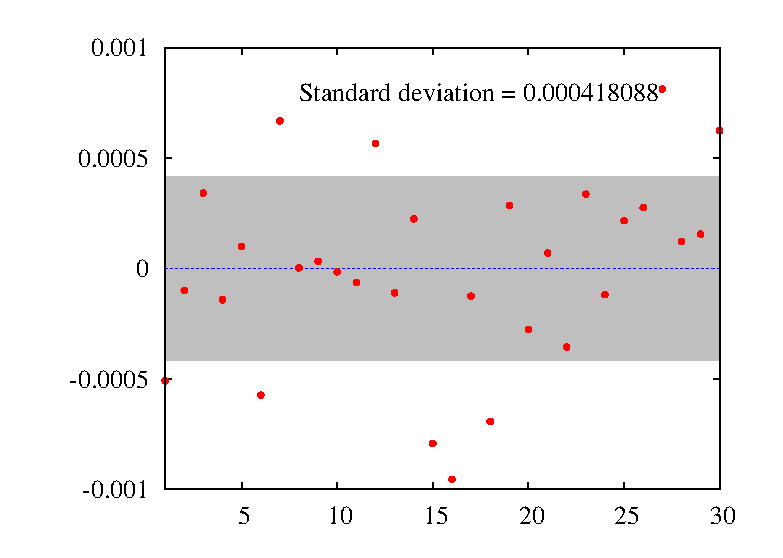
\includegraphics[scale=0.33]{plots/harp-30-miami-percent.eps}}
\caption{Error in counting \textit{U5-1} for 30 interations for Miami.}
\label{fig:miami-30-run}
\end{center}
\end{minipage}
\hfill
\begin{minipage}[t]{0.45\linewidth}
\begin{center}
\centerline{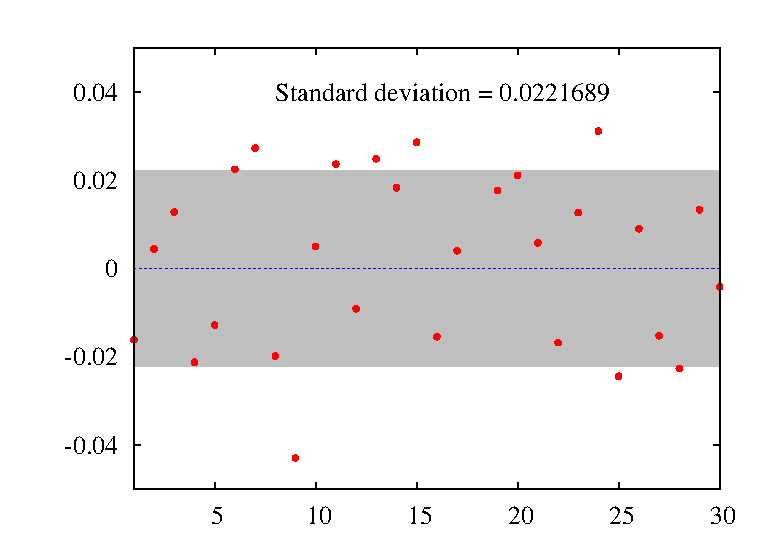
\includegraphics[scale=0.33]{plots/harp-30-webgoogle-percent.eps}}
\caption{Error in counting \textit{U5-1} for 30 interations for Web-Google.}
\label{fig:webgoogle-30-run}
\end{center}
\end{minipage}
\hfill
\end{figure}


In Figure~\ref{fig:error}, we show that the approximation error is below $0.5\%$
for the template \emph{U7-1} for the GNP100 graph, even for one iteration. The
figure also plots the results based on using more than 7 colors, which can
sometimes improve the running time, as discussed in~\cite{huffner2008algorithm}.
In the rest of the experiments, we only use the estimation from one iteration,
because of the small error shown in this section. The error for $i$ iterations
is computed using $\frac{|(\sum_i{Z_i})/i-emb(T,G)|}{emb(T,G)}$.


\begin{figure}[htbp]
\hfill
\begin{minipage}[t]{0.45\linewidth}
\begin{center}
\centerline{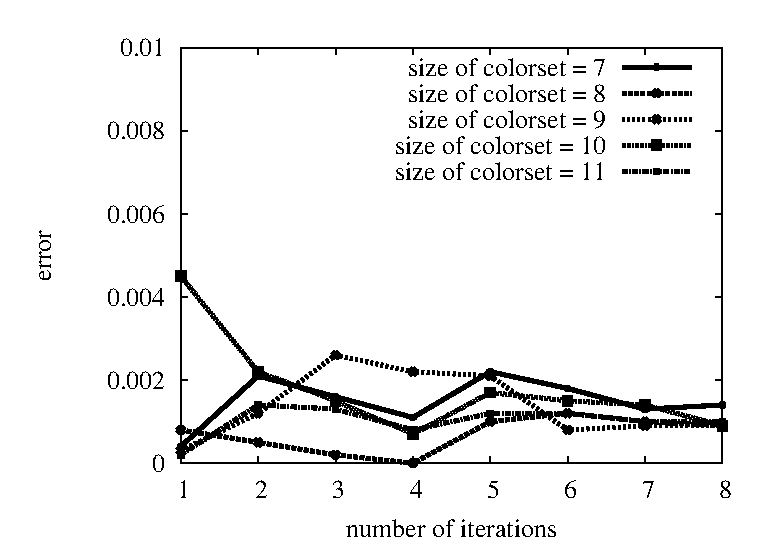
\includegraphics[scale=0.33]{plots/gnpError.eps}}
\caption{Approximation error in counting \emph{U7-1} on GNP100.}
\label{fig:error}
\end{center}
\end{minipage}
\hfill
\begin{minipage}[t]{0.45\linewidth}
\begin{center}
\centerline{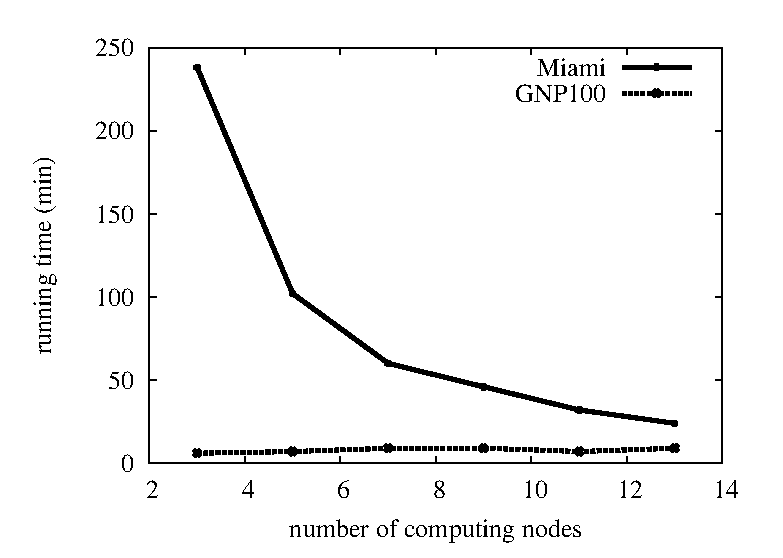
\includegraphics[scale=0.33]{plots/nodes-scale.eps}}
\caption{Running time for counting \textit{U10-1} vs number of computing nodes.}
\label{fig:nodes-scale}
\end{center}
\end{minipage}
\hfill
\end{figure}



\subsubsection{Performance Analysis}
\label{sec:perf}

We now study how the running time is affected by the number of total computing
nodes and number of reducers/mappers per node. We carry out 3 sets of
experiments: (i) how the total running time scales with the number of computing
nodes; (ii) how the running time is affected by varying assignment of
mappers/reducers per node.

\smallskip
\textbf{1. Varying number of computing nodes}
Figure~\ref{fig:nodes-scale} shows that the running time for Miami
reduces from over 200 minutes to less than 30 minutes when the number of
computing nodes increases from 3 to 13. However, the curve for GNP100 does not
show good scaling. The reason is that the actual computation for GNP100 only
consumes a small portion of the running time, and there are overheads from
managing the mappers/reducers. In other words, the curve for GNP100 shows a
lower bound on the running time in our algorithm.

\smallskip
\textbf{2.Varying number of mappers/reducers per node}
We consider two cases.

\smallskip
\textit{2.a. Varying number of reducers per node}
Figure~\ref{fig:reducer-scale} and
~\ref{fig:reducer-scale-timeslice} show the running time on Athena when we vary
the number of reducers per node. Here we fix the number of nodes to be 16 and
the number of mappers per node to be 4. We find that running $3$ reducers
concurrently on each node minimizes the total running time. From Figure~\ref{fig:reducer-scale-timeslice}
we find that though increasing the number of
reducers per node can reduce the time for the Reduce stage for a single job,
the running time increases sharply in Map and Shuffle stage. As a result,
the total running time increases with the number of reducers. It is because
of the I/O bottleneck for concurrent accessing on Athena, since Athena has only
1 disk per node. This phenomena is not seen on EC2, as seen from
Figure~\ref{fig:amazon-reducer-scale}, indicating that EC2 is
better optimized for  concurrent disk accessing for cloud usage.

\begin{figure}[htbp]
\hfill
\begin{minipage}[t]{0.45\linewidth}
\begin{center}
\centerline{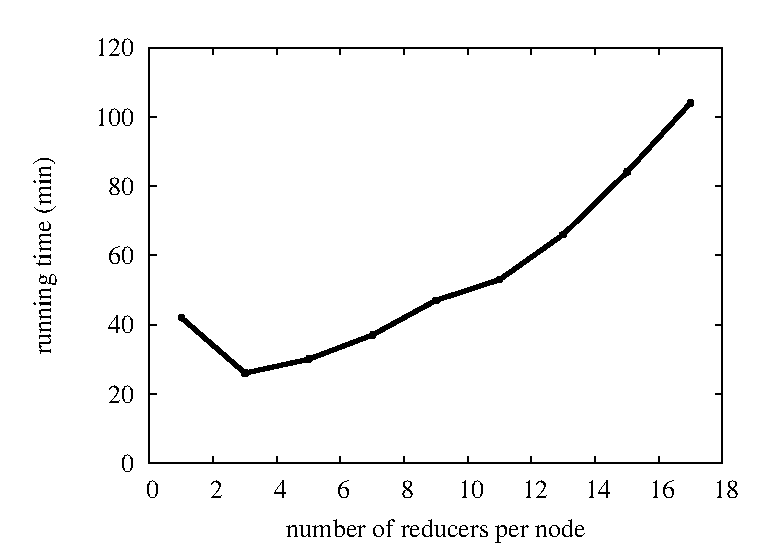
\includegraphics[scale=0.33]{plots/reducer-scale.eps}}
\caption{Total running time versus number of reducers per node.}
\label{fig:reducer-scale}
\end{center}
\end{minipage}
\hfill
\begin{minipage}[t]{0.45\linewidth}
\begin{center}
\centerline{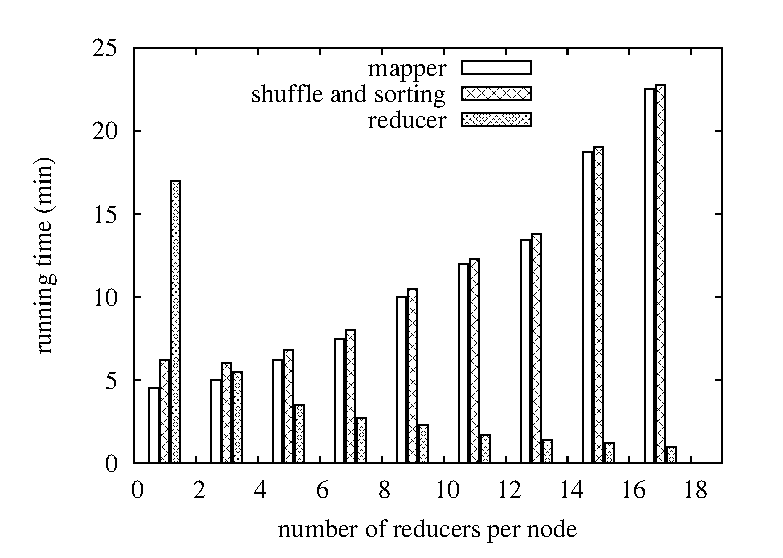
\includegraphics[scale=0.33]{plots/reducer-scale-timeslice.eps}}
\caption{Running time of different job stages versus the number of reducers per node.}
\label{fig:reducer-scale-timeslice}
\end{center}
\end{minipage}
\hfill
\end{figure}

\smallskip
\textit{2.b. Varying number of mappers per node}
Figure~\ref{fig:mapper-scale} and \ref{fig:mapper-scale-timeslice} show the
running time on Athena when we vary the number of mappers per node while fixing
the number of reducers as 7 per node. We find that varying the number of mappers
per node does not affect the performance. This is also validated in EC2, as
shown in Figure~\ref{fig:amazon-mapper-scale}.

\begin{figure}[htbp]
\hfill
\begin{minipage}[t]{0.45\linewidth}
\begin{center}
\centerline{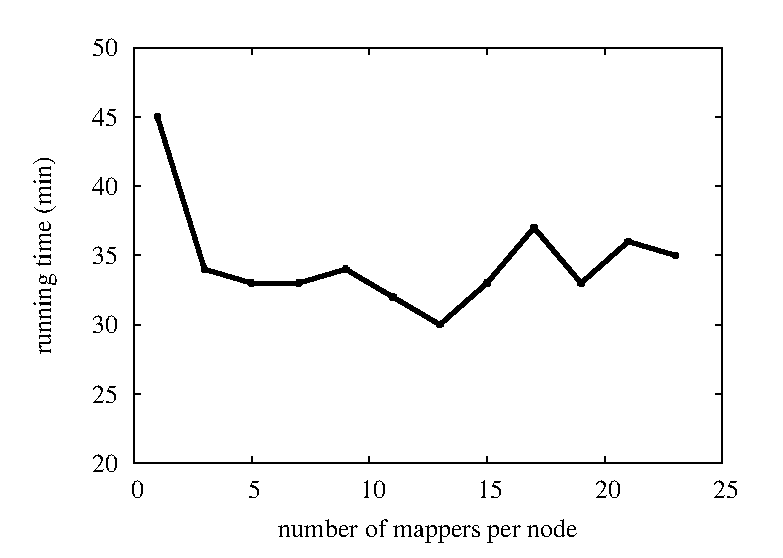
\includegraphics[scale=0.35]{plots/mapper-scale.eps}}
\caption{Total running time versus the number of mappers per node.}
\label{fig:mapper-scale}
\end{center}
\end{minipage}
\hfill
\begin{minipage}[t]{0.45\linewidth}
\begin{center}
\centerline{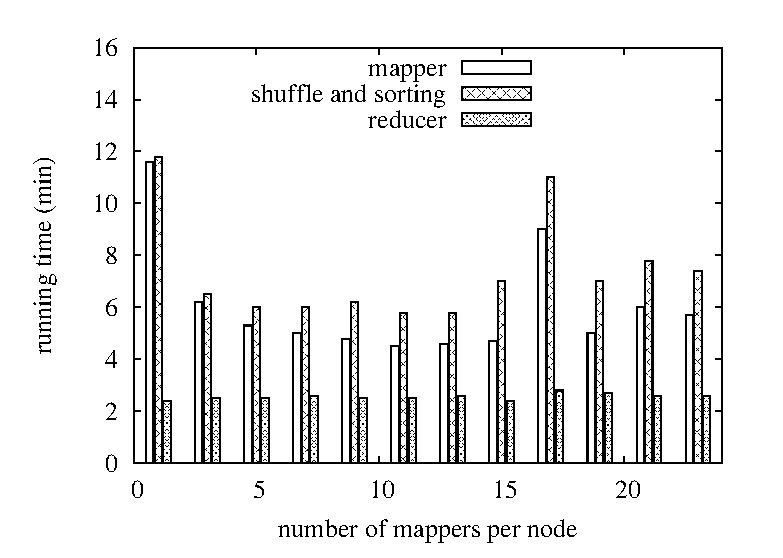
\includegraphics[scale=0.35]{plots/mapper-scale-timeslice.eps}}
\caption{Running time of different job stages versus the number of mappers per node.}
\label{fig:mapper-scale-timeslice}
\end{center}
\end{minipage}
\hfill
\end{figure}

\begin{figure}[htbp]
\hfill
\begin{minipage}[t]{0.45\linewidth}
\begin{center}
\centerline{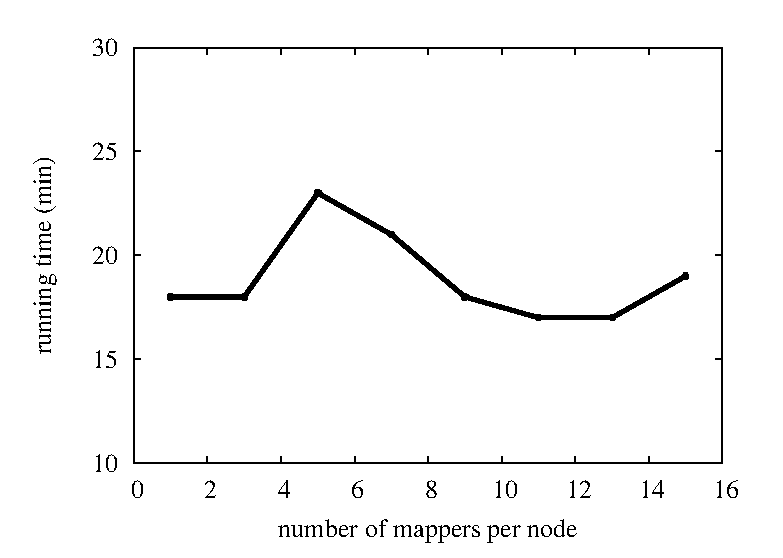
\includegraphics[scale=0.35]{plots/amazon-mapper-scale.eps}}
\caption{Total running time versus number of mappers per node on EC2.}
\label{fig:amazon-mapper-scale}
\end{center}
\end{minipage}
\hfill
\begin{minipage}[t]{0.45\linewidth}
\begin{center}
\centerline{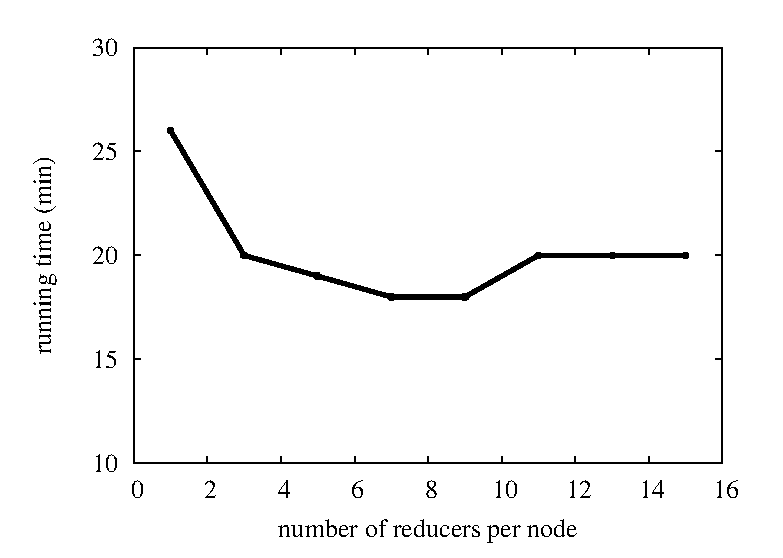
\includegraphics[scale=0.35]{plots/amazon-reducer-scale.eps}}
\caption{Total running time versus number of reducers per node on EC2.}
\label{fig:amazon-reducer-scale}
\end{center}
\end{minipage}
\hfill
\end{figure}

\smallskip
\textit{2.c. Reducers' running time distribution}
Figure~\ref{fig:3reducers-dist}, \ref{fig:7reducers-dist},
~\ref{fig:11reducers-dist} and \ref{fig:15reducers-dist} show the
distribution of the reducers' running time on Athena. We observe that when we
increase the number of reducers per node, the distribution becomes more
volatile; for example, when we concurrently run 15 reducers per node, the reducers'
completion time vary from 20 minutes to 120 minutes. This also indicates the
bad I/O performance on Athena for concurrent accessing.

\begin{figure}[htbp]
\hfill
\begin{minipage}[t]{0.45\linewidth}
\begin{center}
\centerline{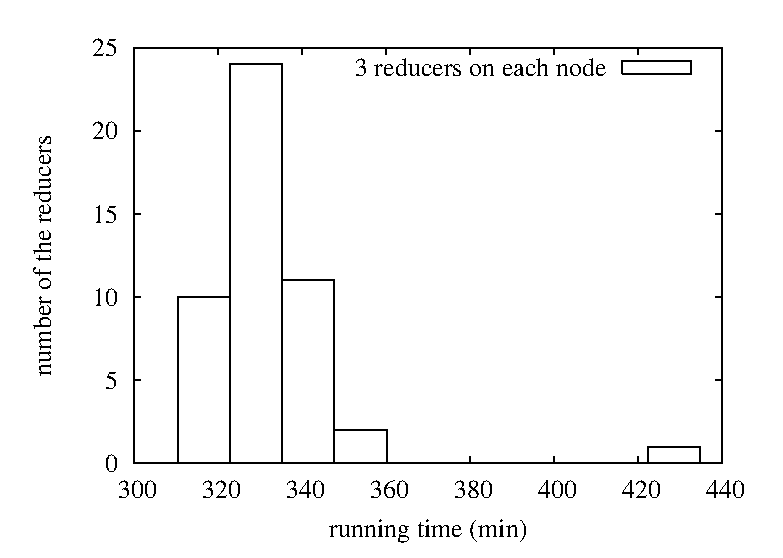
\includegraphics[scale=0.33]{plots/miami-3reducers-dist.eps}}
\caption{3 reducers per computing node.}
\label{fig:3reducers-dist}
\end{center}
\end{minipage}
\hfill
\begin{minipage}[t]{0.45\linewidth}
\begin{center}
\centerline{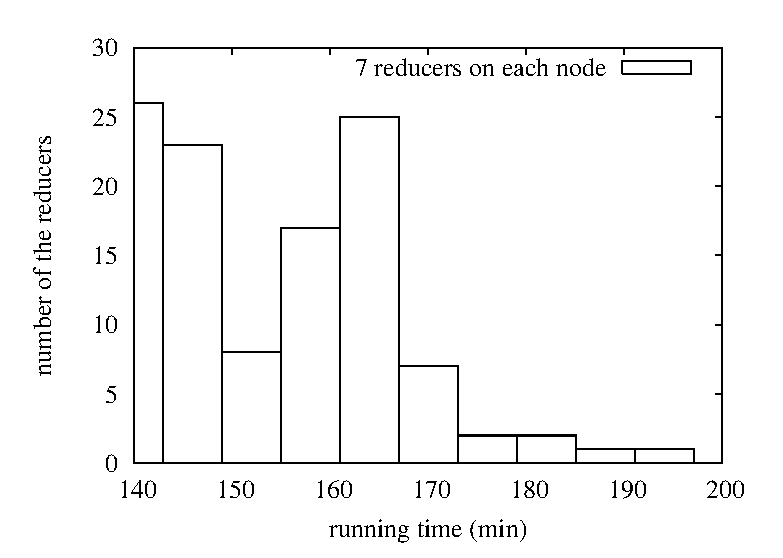
\includegraphics[scale=0.33]{plots/miami-7reducers-dist.eps}}
\caption{7 reducers per computing node.}
\label{fig:7reducers-dist}
\end{center}
\end{minipage}
\hfill
\end{figure}

\begin{figure}[htbp]
\hfill
\begin{minipage}[t]{0.45\linewidth}
\begin{center}
\centerline{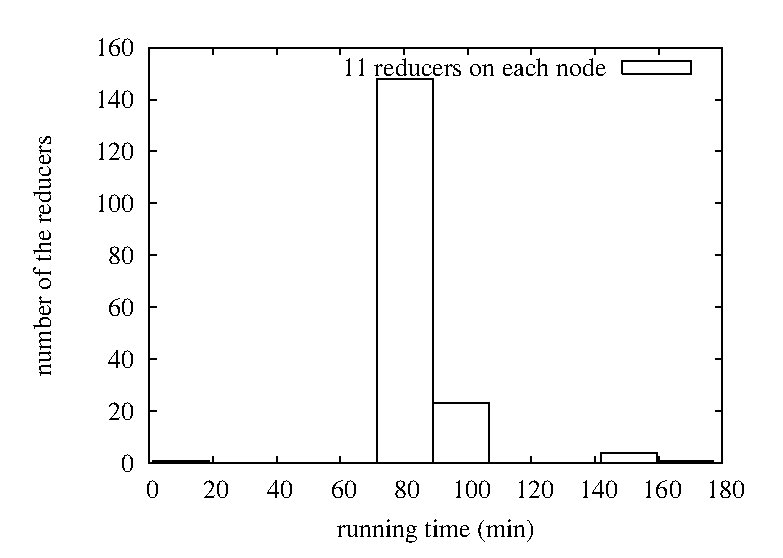
\includegraphics[scale=0.33]{plots/miami-11reducers-dist.eps}}
\caption{11 reducers per computing node.}
\label{fig:11reducers-dist}
\end{center}
\end{minipage}
\hfill
\begin{minipage}[t]{0.45\linewidth}
\begin{center}
\centerline{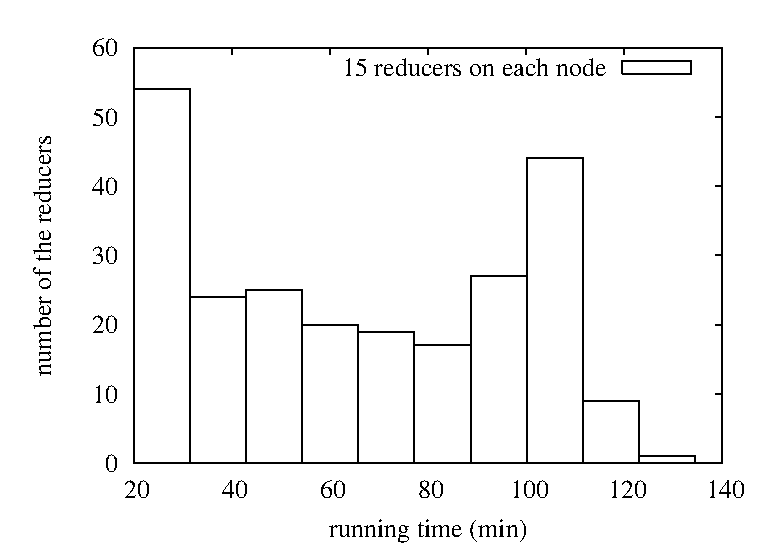
\includegraphics[scale=0.33]{plots/miami-15reducers-dist.eps}}
\caption{15 reducers per computing node.}
\label{fig:15reducers-dist}
\end{center}
\end{minipage}
\hfill
\end{figure}

\iffalse
%%%%%
\textbf{Sizes of the files on HDFS for each sub-template}

Figure~\ref{fig:datasize} shows how the sizes of the files that store the counts
of colorful embeddings vary for different sub-templates when we run on
\textit{U10-1}. It is consistent with the theoretical bound presented in Lemma
~\ref{lemma:counter}.

\begin{figure}[htbp]
\centerline{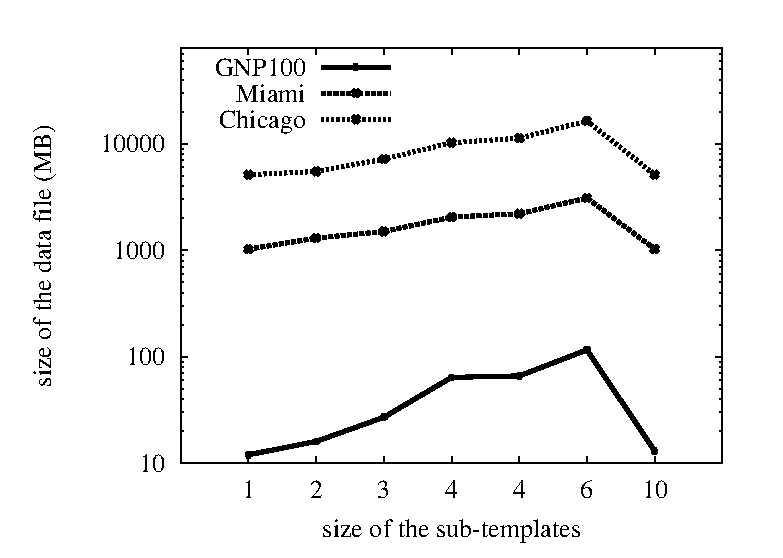
\includegraphics[scale=0.35]{plots/unlabel-sizebound.eps}}

\caption{Size of the data for $\forall T_i \in \mathcal{T}$.  There are totally
7 templates in $\mathcal{T}$, two of which are with the same size 4.}
\label{fig:datasize}
\end{figure}
%%%%%%%
\fi

\subsubsection{Illustrative applications}
In this section, we illustrate the performance on $3$ different kinds of
queries. We use Athena and assign $16$ nodes as the data nodes; for each node,
we assign a maximum of $4$ mappers and $3$ reducers per node. Our experiments
on EC2 for some of these queries are discussed later in
Section~\ref{sec:experiments-ec2}.

\smallskip
\textbf{1. Unlabeled subgraph queries:} Here we compute the counts of
templates \emph{U5-1}, \emph{U7-1} and \emph{U10-1} on GNP100 and Miami, as
shown in Figure~\ref{fig:unlabel-counts}. We also plot how the running time
scales to different templates and networks, as shown in Figure
~\ref{fig:unlabel-time} -- we observe that for unlabeled template with up to
$10$ nodes on the Miami graph, the algorithm runs in less than $25$ minutes.

\begin{figure}[htbp]
\hfill
\begin{minipage}[t]{0.45\linewidth}
\begin{center}
\centerline{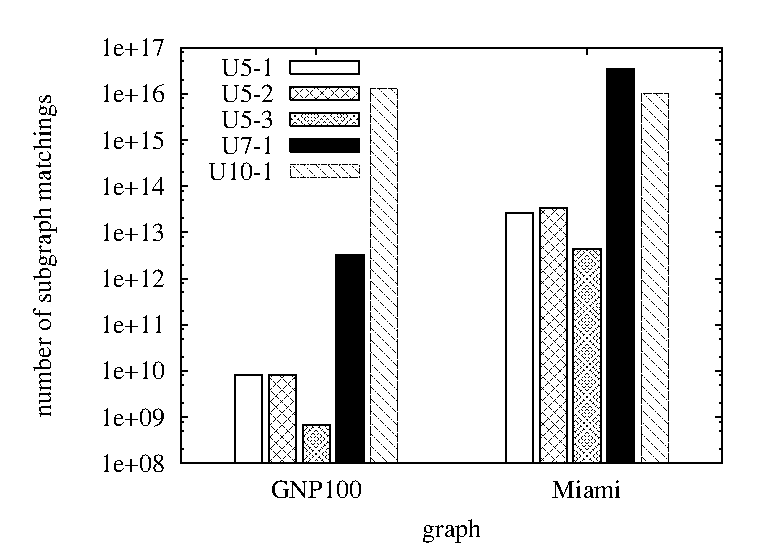
\includegraphics[scale=0.35]{plots/unlabel-count.eps}}
\caption{The counts of unlabeled subgraphs in GNP100 and Miami.}
\label{fig:unlabel-counts}
\end{center}
\end{minipage}
\hfill
\begin{minipage}[t]{0.45\linewidth}
\begin{center}
\centerline{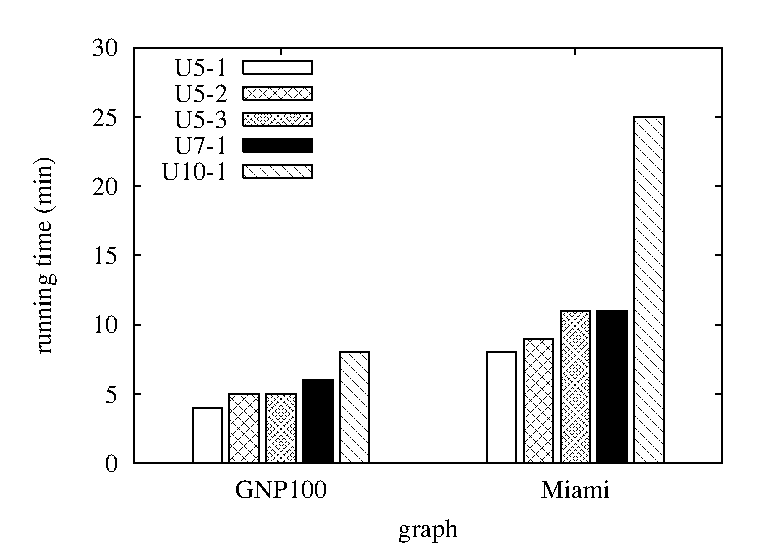
\includegraphics[scale=0.35]{plots/unlabel-time.eps}}
\caption{Running time for counting unlabeled subgraph in GNP100 and Miami.}
\label{fig:unlabel-time}
\end{center}
\end{minipage}
\hfill
\end{figure}

\smallskip
\textbf{2. Labeled subgraph queries:} Here we count the total number of
embeddings of template \emph{L7-1}, \emph{L10-1} and \emph{L12-1} in Miami and
Chicago. Figure~\ref{fig:label-time} shows that the running time for counting
templates up to $12$ nodes is around $15$ minutes on Miami, less than $35$
minutes needed for Chicago. The running time is much less for the labeled
subgraph queries than that for the unlabeled subgraph queries. It is due to the
fact that that labeled templates have much less number of embeddings due to the
label constraints.

\begin{figure}[htbp]
\hfill
\begin{minipage}[t]{0.45\linewidth}
\begin{center}
\centerline{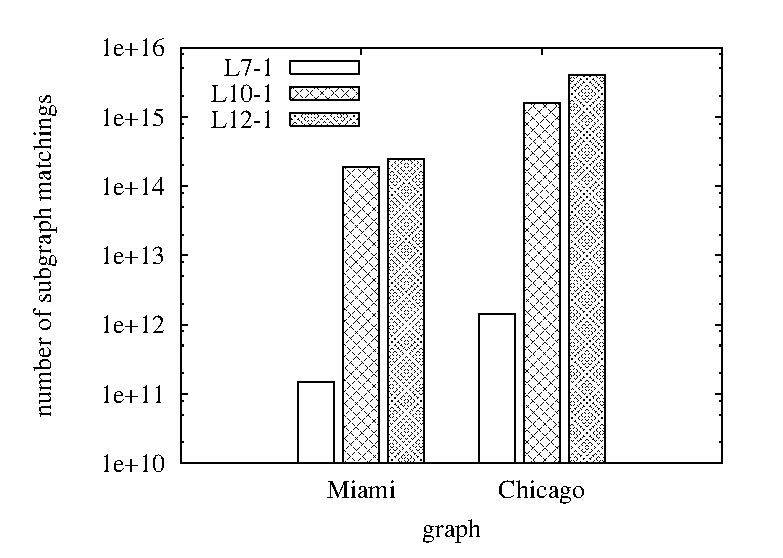
\includegraphics[scale=0.35]{plots/label-count.eps}}
\caption{The counts of labeled templates in Miami and Chicago.}
\label{fig:label-count}
\end{center}
\end{minipage}
\hfill
\begin{minipage}[t]{0.45\linewidth}
\begin{center}
\centerline{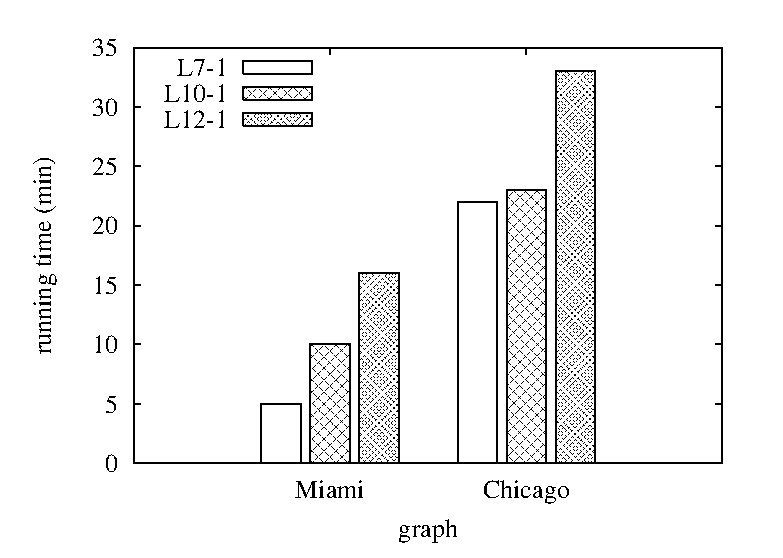
\includegraphics[scale=0.35]{plots/label-time.eps}}
\caption{Running time for counting labeled templates in Miami and Chicago.}
\label{fig:label-time}
\end{center}
\end{minipage}
\hfill
\end{figure}

\smallskip
\textbf{3. Computing graphlet frequency distribution:} Figure
~\ref{fig:miami-graphlet} and \ref{fig:chicago-graphlet} show the graphlet
frequency distribution of the networks of Miami and Chicago, respectively. The
template is \emph{U5-1}. It takes 15 minutes and 35 minutes to compute graphlet
frequency distribution on Miami and Chicago, respectively.

\begin{figure}[htbp]
\hfill
\begin{minipage}[t]{0.45\linewidth}
\begin{center}
\centerline{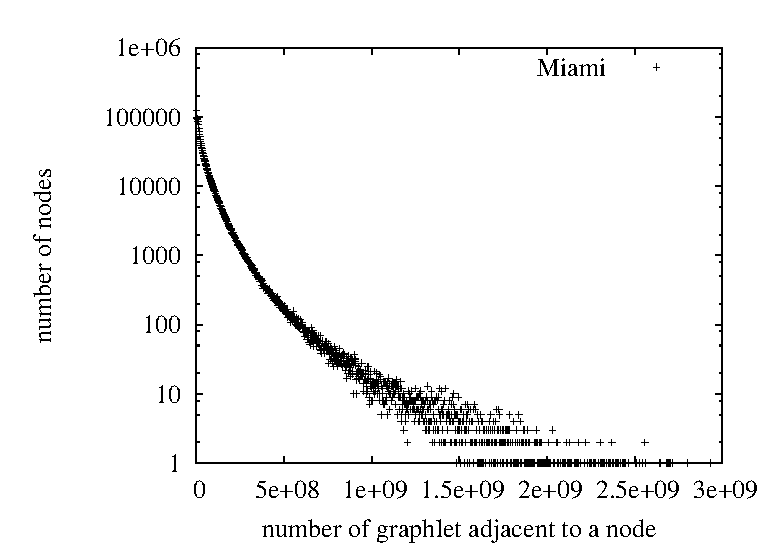
\includegraphics[scale=0.35]{plots/miami-graphlet.eps}}
\caption{Graphlet frequency distribution of Miami.}
\label{fig:miami-graphlet}
\end{center}
\end{minipage}
\hfill
\begin{minipage}[t]{0.45\linewidth}
\begin{center}
\centerline{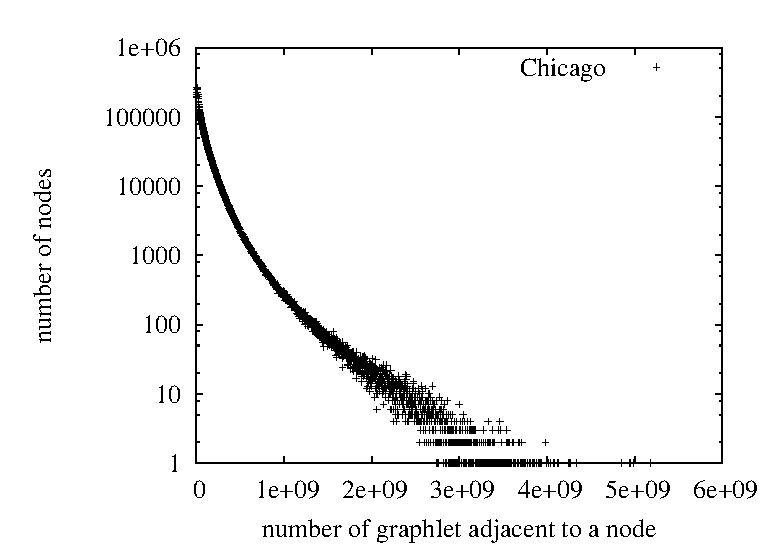
\includegraphics[scale=0.35]{plots/chicago-graphlet.eps}}
\caption{Graphlet frequency distribution of Chicago.}
\label{fig:chicago-graphlet}
\end{center}
\end{minipage}
\hfill
\end{figure}




\subsubsection{Performance Study with Amazon EC2}
\label{sec:experiments-ec2}

On EC2, we run unlabeled and labeled subgraph queries on Miami and GNP100 for
templates \emph{U5-1}, \emph{U7-1}, \emph{U10-1}, \emph{L7-1}, \emph{L10-1} and
\emph{L12-1}. We use the same $4$ EC2 instances as discussed previously, and
each node runs up to a maximum of $2$ mappers and $8$ reducers concurrently. As
shown in Figures~\ref{fig:amazon-gnp-time} and~\ref{fig:amazon-miami-time.eps},
the running time on EC2 is comparable to that on Athena, except for
\emph{U10-1} on Miami, which takes roughly $2.5$ hours to finish on EC2, but
only $25$ minutes on Athena. This is because for such a large template and
graph as large as Miami, input/output data as well as the I/O pressure on disks
are tremendous. EC2 uses virtual disks as local storage, which hurt overall
performance when dealing with such a large amount of data.

\begin{figure}[htbp]
\hfill
\begin{minipage}[t]{0.45\linewidth}
\begin{center}
\centerline{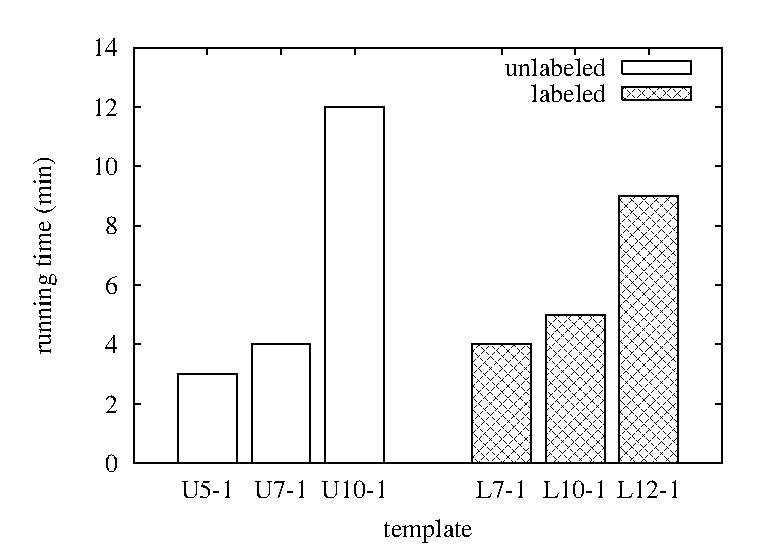
\includegraphics[scale=0.35]{plots/amazon-gnp-time.eps}}
\caption{Running time for various templates on GNP100.}
\label{fig:amazon-gnp-time}
\end{center}
\end{minipage}
\hfill
\begin{minipage}[t]{0.45\linewidth}
\begin{center}
\centerline{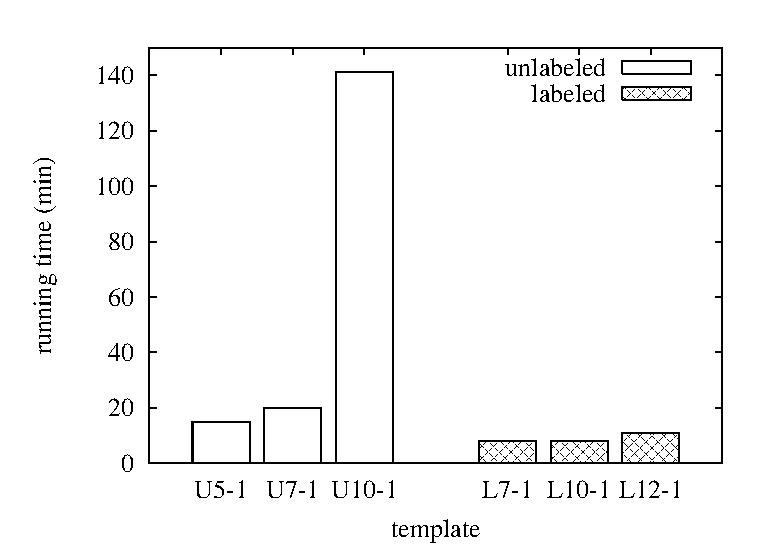
\includegraphics[scale=0.35]{plots/amazon-miami-time.eps}}
\caption{Running time for various templates on Miami.}
\label{fig:amazon-miami-time.eps}
\end{center}
\end{minipage}
\hfill
\end{figure}



\subsection{Performance of \ensahad{}}
\label{sec:exp:enhanced-sahad}


In this section we experiment our algorithms on two real-world networks
\textit{nrv} and \textit{rNet} and a number of their shuffled versions. We
generate shuffled networks with 20, 40, 60, 80 and 100 percent shuffling ratio.
, and name them as \textit{nrv20} to \textit{nrv100}, and \textit{rNet20} to
\textit{rNet100}. 

%The purpose of using shuffled networks is to study the impact
%of the randomness on $E_{out}$ and performance.

%\subsubsection{Reducing Intermediate Cost with Pre-allocated Reducers}
As discussed in Section~\ref{sec:ensahad}, a major factor that impact the
overall performance is the heavy shuffling and sorting cost in the intermediate
stage of a Hadoop job. We mitigate this factor by designating node index $v$ to
Reducers, and pre-allocate Reducers among computing nodes. In such a way, the
key-value pairs from Mappers can be directly sent to corresponding Reducers
without being shuffled and sorted.  

Figures~\ref{fig:enhanced-sahad-sorting-nrv} and
~\ref{fig:enhanced-sahad-sorting-rnet} show the overall running time of our
algorithm on \textit{NRV}, \textit{RoadNet} and their variations. Here we
generate the variations of the graph by shuffling a proportion of the edges in
the graph, e.g., \textit{nrv40} is a \textit{NRV} with 40\% of its edges being
shuffled. We see that pre-allocating Reducer can bring roughly 20\% performance
improvement.  

\begin{figure}[htbp]
\hfill
\begin{minipage}[t]{0.45\linewidth}
\begin{center}
\centerline{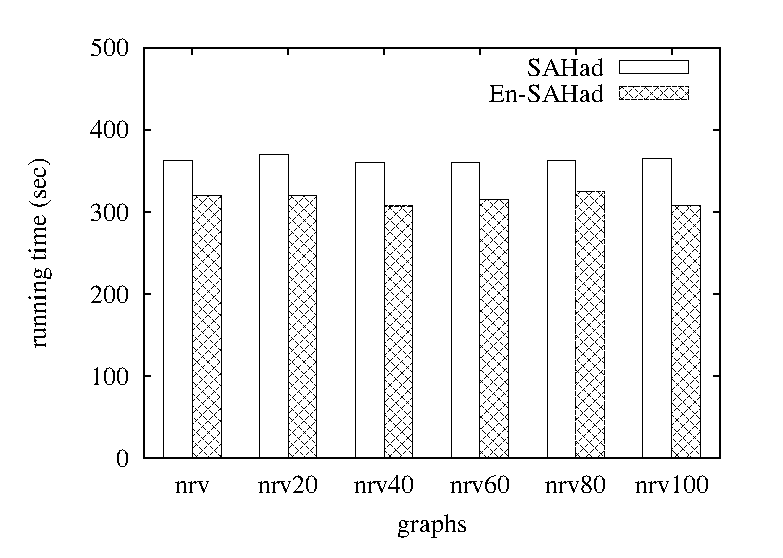
\includegraphics[scale=0.35]{plots/enhanced-sahad-sorting-nrv.eps}}
\caption{\sahad{} vs \ensahad{} on NRV and its variations}
\label{fig:enhanced-sahad-sorting-nrv}
\end{center}
\end{minipage}
\hfill
\begin{minipage}[t]{0.45\linewidth}
\begin{center}
\centerline{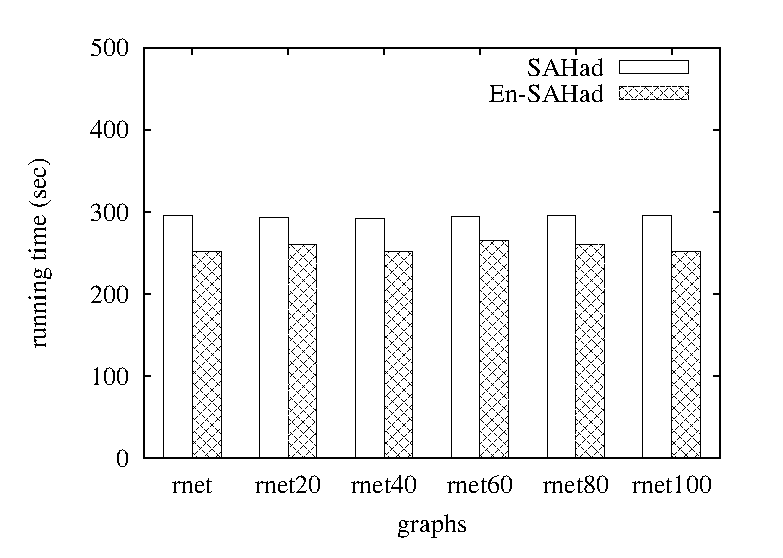
\includegraphics[scale=0.35]{plots/enhanced-sahad-sorting-rnet.eps}}
\caption{\sahad{} vs \ensahad{} on RoadNet and its variations}
\label{fig:enhanced-sahad-sorting-rnet}
\end{center}
\end{minipage}
\hfill
\end{figure}

\iffalse
\subsubsection{Communication cost among computing nodes}
\label{sec:exp:partition}

Real world networks tend to have nodes connected in the form of communities,
e.g., in social networks, a group of nodes tends to have more internal
connections among them and much less connections among groups~\cite{girvan2002community}.
Therefore, by performing minimum cut partitioning on such
networks, the number of inter-partition edges $E_{out}$ are expected to be much less than
performing random partition schemes on those networks. E.g. Figure~\ref{fig:nrv-random-min-cut-edges}
shows that the number of inter-partition edges are
much less in min-cut based for \textit{NRV} than in random based
partitions. It is also observed that the more the randomness brought into the
network, the less of the difference. This complies with our assumption that
min-cut partitioning has a larger effect in terms of number of inter-partition
edges on real world networks than random networks due to the community effect.

\begin{figure}[htbp]
\hfill
\begin{minipage}[t]{0.45\linewidth}
\begin{center}
\centerline{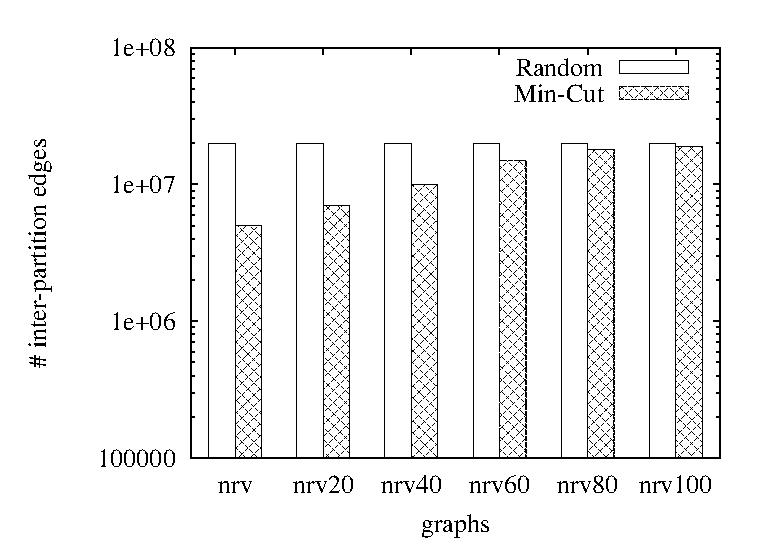
\includegraphics[scale=0.35]{plots/enhanced-sahad-inter-part-nrv.eps}}
\caption{Number of inter-partition edges in min-cut and random partitions for \textit{NRV}}
\label{fig:nrv-random-min-cut-edges}
\end{center}
\end{minipage}
\hfill
\begin{minipage}[t]{0.45\linewidth}
\begin{center}
\centerline{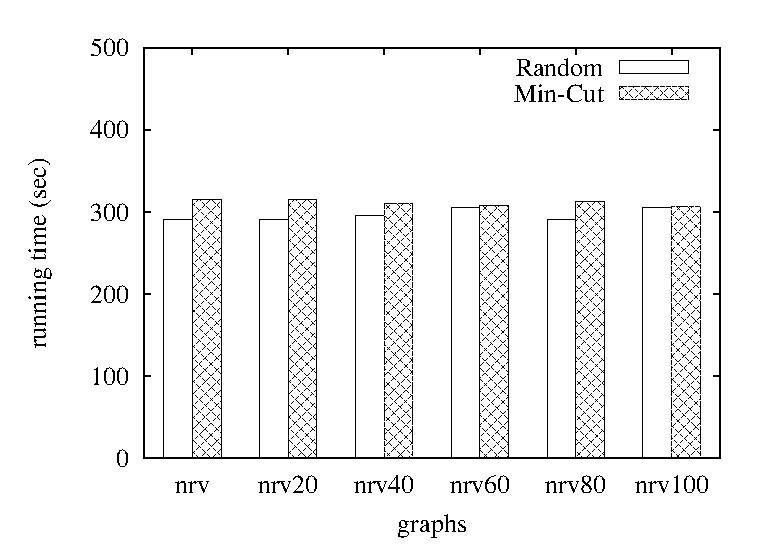
\includegraphics[scale=0.35]{plots/enhanced-sahad-inter-part-nrv-time.eps}}
\caption{Running time comparison with min-cut and random partitions for
\textit{NRV}}
\label{fig:nrv-random-min-cut-time}
\end{center}
\end{minipage}
\hfill
\end{figure}

Figure~\ref{fig:nrv-random-min-cut-time} shows the total running time of
applying different partitioning schemes on \textit{nrv} and its variations. As
observed the total running time does not vary significantly between different
partitioning schemes. The reason is that although min-cut based partitioning
scheme may reduce the communication cost among partititions in enhanced
\sahad{}, however, the increased number of intra-partition edges may
actually increase the computational cost in subgraph counting within a
partition. 

\fi







\subsection{Performance of \harpsahad{}}
\label{sec:exp:harp}
In this section, we discuss the performance of \harpsahad{} and compare its performance
with \sahad{}. 

\subsubsection{\harpsahad{} versus \sahad{}} 
For network Web-Google, \harpsahad{} runs about 5 times faster than \sahad{}; and for
network Miami, \harpsahad{} runs about 9 times faster than Sahad. In addition,
Figure~\ref{fig:harp-vs-sahad} shows high efficiency in implementations — the
total execution time increases 2 times when the graph dataset increases to
about 11 times from Web-Google to Miami. 


\begin{figure}[htbp]
\hfill
\begin{minipage}[t]{0.45\linewidth}
\begin{center}
\centerline{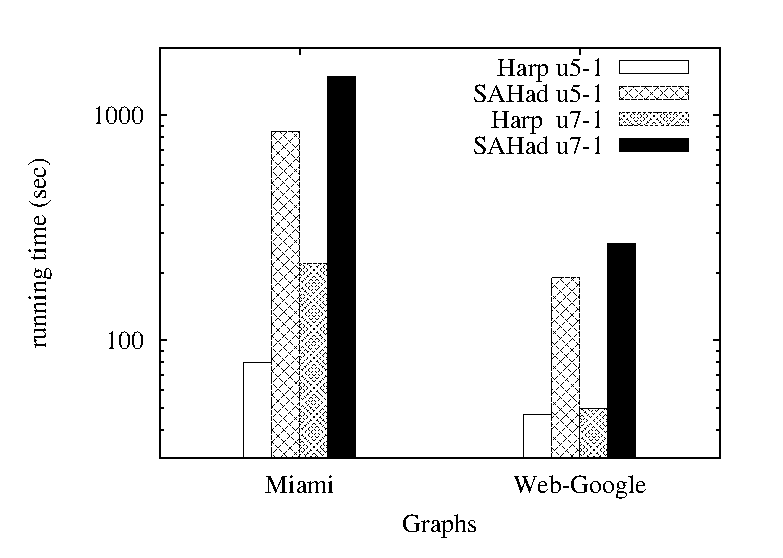
\includegraphics[scale=0.35]{plots/harp-vs-sahad-40-threads.eps}}
\caption{Comparing the running times  of \harpsahad{} and \sahad{} on templates
\textit{u5-1} and \textit{u7-1}.}
\label{fig:harp-vs-sahad}
\end{center}
\end{minipage}
\hfill
\begin{minipage}[t]{0.45\linewidth}
\begin{center}
\centerline{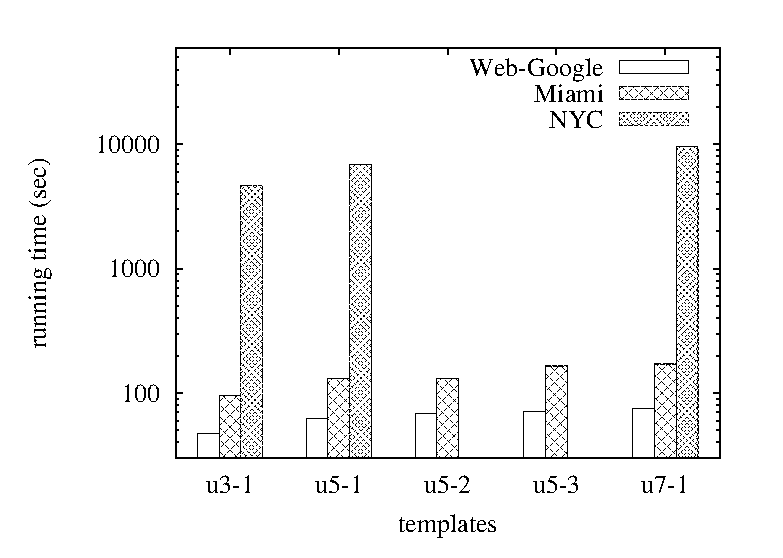
\includegraphics[scale=0.35]{plots/harp-varying-templates-4-nodes-40-threads.eps}}
\caption{Running time of \harpsahad{} with different templates and graphs.}
\label{fig:harp-varying-templates}
\end{center}
\end{minipage}
\hfill
\end{figure}

\subsubsection{Scalability of \harpsahad{}}

In this section, we discuss how Harp performs with different templates and
graphs. We start our experiment by running Harp against different templates with
$|k|$ from 3 to 7, and on 4 graphs with number of nodes varying from 0.9
millions to 41 millions. Figure~\ref{fig:harp-varying-templates} shows that the
computational cost on Harp is more sensitive to the size of the graph than the
size of the templates.    


Then we studies the performance by controlling the number of nodes in a graph and
increase the number of edges. Here we use Chung-Lu model~\cite{aiello2000random}
to generate a series of random graphs given the degree sequence and its
variations of Miami and NYC.  The average degree of generated random graphs
ranging from 50 to 150 for Miami and 10 to 100 for NYC. As we can see from
Figure~\ref{fig:harp-cl-miami} and Figure~\ref{fig:harp-cl-nyc}, generally the
running time increases according to the number of edges of the graph, which
meets the time complexity we propose in Section~\ref{sec:performance-analysis}.
Specifically, the running time on the Chung-Lu graphs based off NYC shows a
quadratic curve with increasing number of edges, which matches Equation
~\ref{eq:total-time}. The results on Miami does not show quadratic increase
due to the relative small computational cost comparing to other overhead of the
system.  


\begin{figure}[htbp]
\hfill
\begin{minipage}[t]{0.45\linewidth}
\begin{center}
\centerline{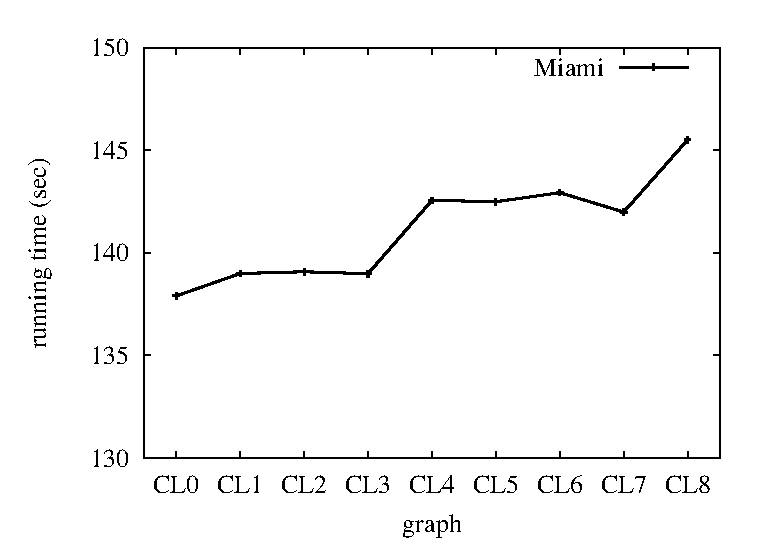
\includegraphics[scale=0.35]{plots/harp-cl-miami.eps}}
\caption{Running time of \harpsahad{} given a series of Chung-Lu random graph \
based off \textit{Miami} with increasing number of edges.}
\label{fig:harp-cl-miami}
\end{center}
\end{minipage}
\hfill
\begin{minipage}[t]{0.45\linewidth}
\begin{center}
\centerline{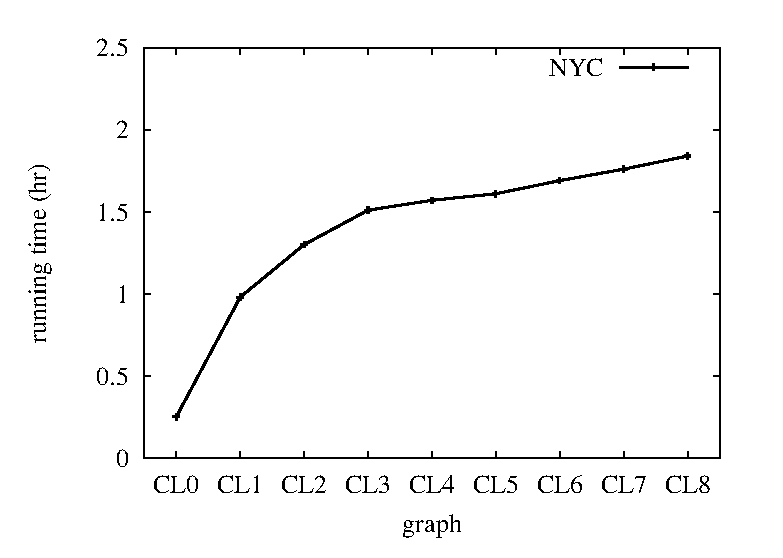
\includegraphics[scale=0.35]{plots/harp-cl-nyc.eps}}
\caption{Running time of \harpsahad{} given a series of Chung-Lu random graph \
based off \textit{NYC} with increasing number of edges.}
\label{fig:harp-cl-nyc}
\end{center}
\end{minipage}
\hfill
\end{figure}


\subsubsection{Varying number of computing nodes}


\begin{figure}[htbp]
\hfill
\begin{minipage}[t]{0.45\linewidth}
\begin{center}
\centerline{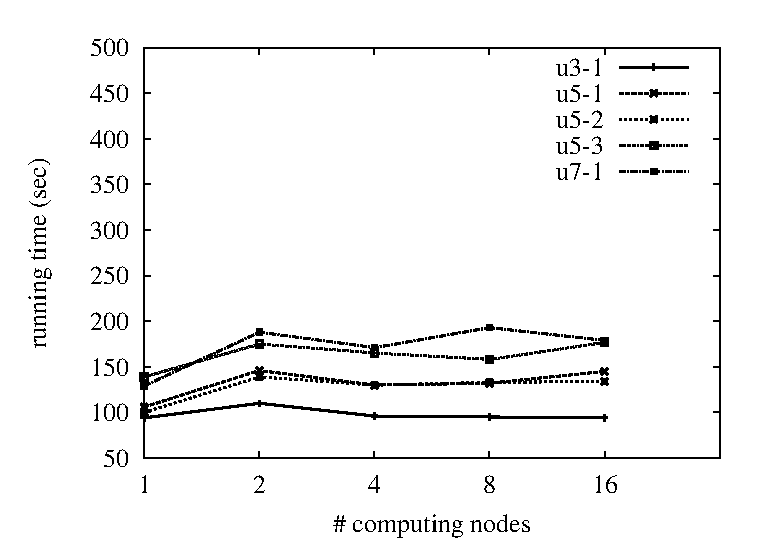
\includegraphics[scale=0.35]{plots/harp-varying-nodes-templates-40-threads-miami.eps}}
\caption{Running time of \harpsahad{} given different number of computing nodes and templates on Miami}
\label{fig:harp-varying-nodes-templates-miami}
\end{center}
\end{minipage}
\hfill
\begin{minipage}[t]{0.45\linewidth}
\begin{center}
\centerline{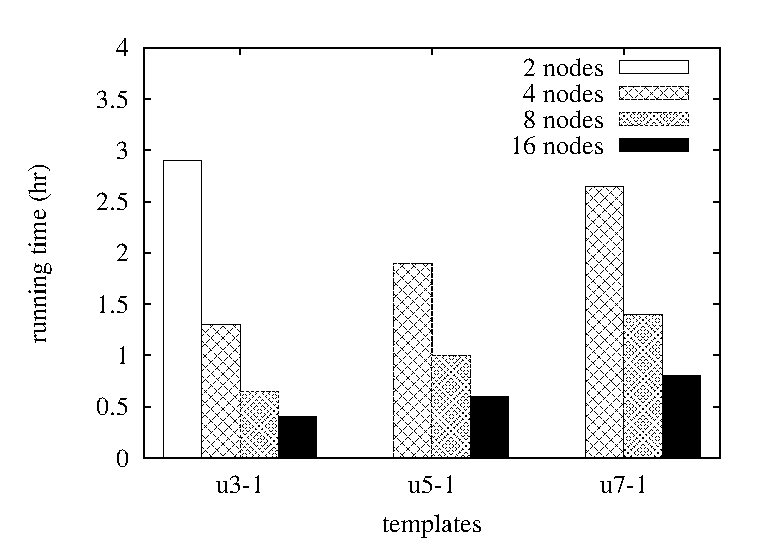
\includegraphics[scale=0.35]{plots/harp-nyc-varying-nodes.eps}}
\caption{Running time on NYC scales with number of computing nodes}
\label{fig:harp-nyc-varying-nodes}
\end{center}
\end{minipage}
\hfill
\end{figure}

In this section, we study the performance of \harpsahad{} as a function
of computing resources, i.e., computing nodes and threads per node.
Figure~\ref{fig:harp-varying-nodes-templates-miami} shows that for Miami the
performance does not improve with increasing number of the computing nodes. It
is due to the low computation cost within each nodes and high communication
cost. An increasing number of nodes brings in more communication cost that
tradeoffs the gain on computation. To further investigate the performance
challenges on big dataset, we run experiments on the NYC dataset, which is about
9 times larger than the Miami dataset. Figure~\ref{fig:harp-nyc-varying-nodes}
presents the running time on different number of machine nodes (2, 4, 8 and 16
nodes). It clearly shows a good scalability of the Harp implementation.  

\iffalse
%%%%%%%
We
further break down the execution cost with two experiments as shown in Figure
~\ref{fig:harp-time-breakdown}: i) running with template u3-1 on 8 nodes; ii)
running with template u3-1 on 16 nodes. The total communication time takes about
77\% of the execution time in the experiments, which indicates that our
algorithm is intensive on communication.

\begin{figure}[htbp]

\centerline{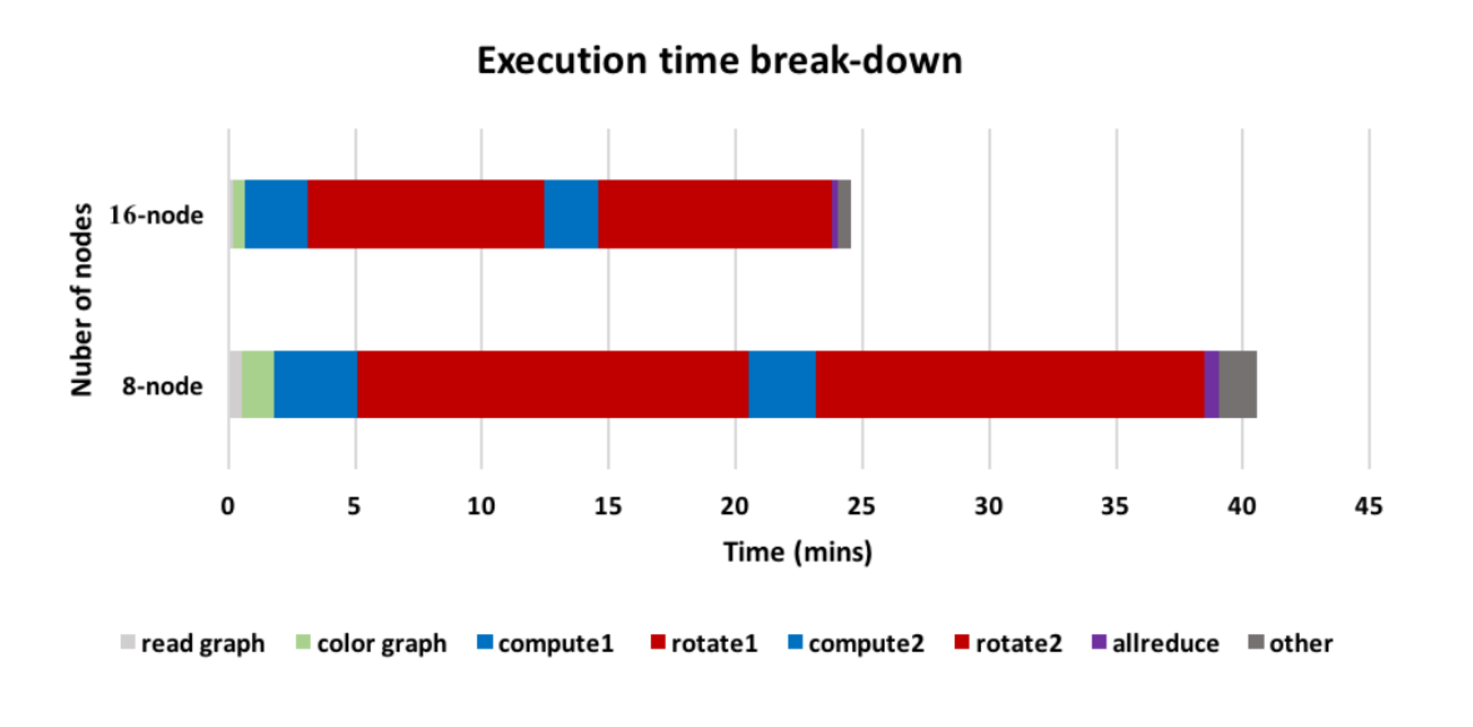
\includegraphics[width=0.50\textwidth]{plots/harp-time-breakdown.eps}}

\caption{The running time breakdown of Harp on NYC. Rotate1 and Rotate2
represents communication time and occupies 77\% of total running time.}

\label{fig:harp-time-breakdown}
\end{figure}
%%%%%%%%
\fi



\subsubsection{Degree based partitioning schemes}
In the above experiments, we evenly partition the graphs without considering the
nature of the problem and the structure of the graphs. With that, each partition
has the same number of nodes. 

In this section, we experiment a new partition scheme based on a degree-related
metric $D_p$ as shown in Equation~\ref{eq:degree2-partition}. Given a node with
degree $d$, there are totally $d \choose 2$ different pairs of edges that
sub-templates $\tau'$ and $\tau''$ can resides at, or $O(d^2)$ ways to join 2
sub-templates. To have roughly equal computational cost within each partition
$p$ we partition the graph such that each partition has similar $D_p$. We expect
that the computation in each partition will be roughly the same with this
partitioning scheme, therefore there is less overhead in synchronization and
unbalanced load.

\begin{equation}
\label{eq:degree2-partition}
\displaystyle D_p = \sum_{\forall v \in p}{{d_v}^2}
\end{equation}

Here $d_v$ is the degree of node $v$. 

\iffalse
%%%%%%%%
\begin{figure}[htbp]

\centerline{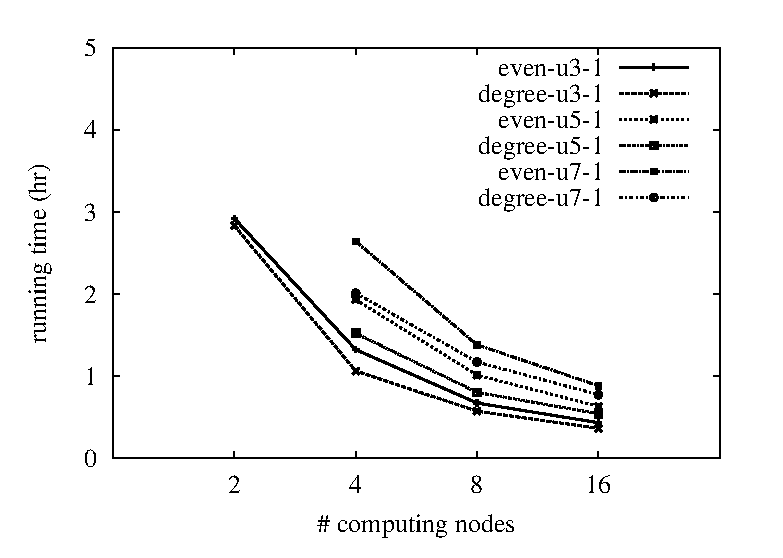
\includegraphics[width=0.40\textwidth]{plots/harp-degree2-nyc.eps}}

\caption{Degree based partitioning scheme gives a 20\% increase in running time
over even partitioning}

\label{fig:harp-degree2-nyc}
\end{figure}


Figure~\ref{fig:harp-degree2-nyc} indicates that the $D_p$ based partitioning
scheme can bring up to 20\% improvement to the performance of our Harp
implementation.
%%%%%%%
\fi


\begin{figure}[htbp]
\hfill
\begin{minipage}[t]{0.45\linewidth}
\begin{center}
\centerline{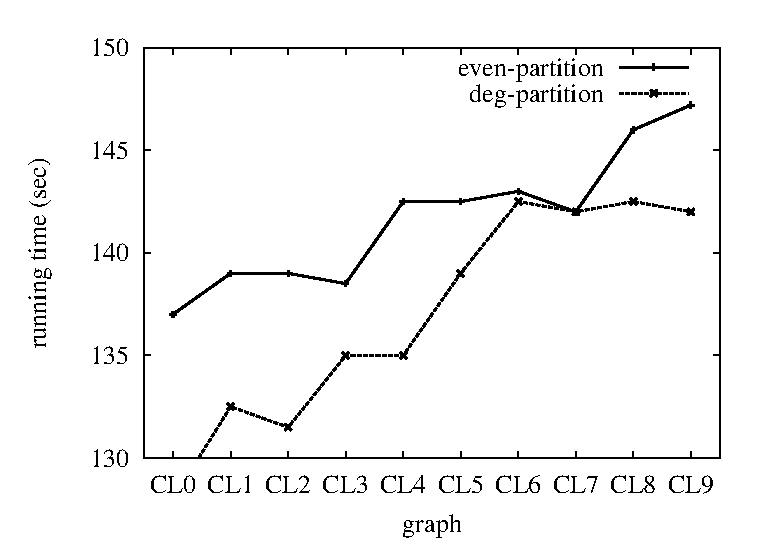
\includegraphics[scale=0.35]{plots/harp-degree2-miami-cl.eps}}
\caption{Running time of Harp on Miami with even and degree based partitioning}
\label{fig:harp-degree2-miami-cl}
\end{center}
\end{minipage}
\hfill
\begin{minipage}[t]{0.45\linewidth}
\begin{center}
\centerline{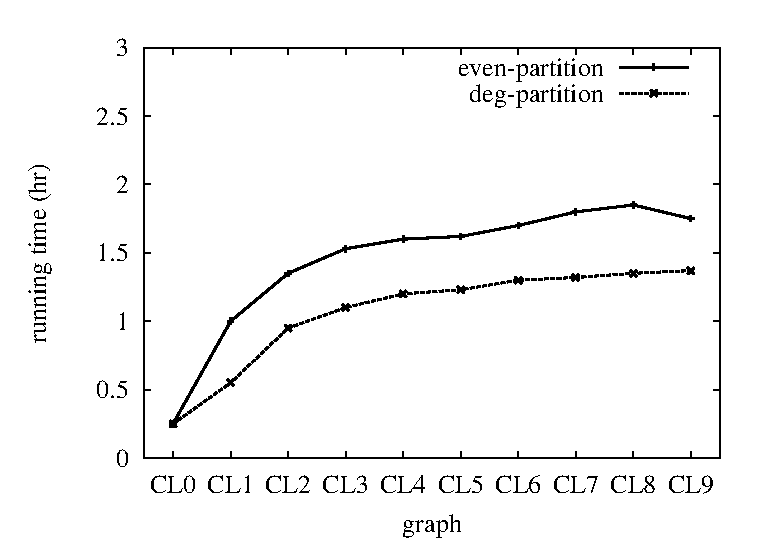
\includegraphics[scale=0.35]{plots/harp-degree2-nyc-cl.eps}}
\caption{Running time of Harp on NYC with even and degree based partioning}
\label{fig:harp-degree2-nyc-cl}
\end{center}
\end{minipage}
\hfill
\end{figure}

Figures~\ref{fig:harp-degree2-miami-cl} and~\ref{fig:harp-degree2-nyc-cl} show
the performance gain obtained by partitioning the graph based on $D_p$. We
noticed that on Miami, the performance improvement is merely 3\%, which is
largely due to the relatively small size of the graph and computational cost.
However, degree based partitioning improve the performance on NYC by an average
of 21\%, showing that for larger graphs that can incur high computational cost,
how the graph is partitioned plays a major role.

